%! TEX root = main.tex

\graphicspath{{00_Images/06_chapter/}}

\chapter{Mixing Console Architecture and Electronics}
\label{ch:mixingconsole}

\section{General Architecture and Signal Flow}
\label{sc:61}

A mixing console is the central hub of any recording or live-sound system, responsible for accepting signals from multiple sources, processing them individually, combining them into a coherent mix, and routing the result to the outputs.
Although the specific layout varies across manufacturers and product lines, the underlying electronic architecture is substantially common to all professional analog desks.
The Soundcraft Series FIVE serves as a representative reference throughout this chapter: it is a large-format console designed for both live and studio use, and its input module exemplifies the canonical signal path found in professional analog mixing.

\subsection{The Mono Input Module}
\label{sc:611}

The signal path through a mono input channel begins at the XLR/jack input connector and proceeds through a sequence of well-defined processing stages before reaching the mix bus.
Understanding each stage and its position in the chain is essential for operating the console correctly and for diagnosing signal-flow problems in a real session.

% SUGGESTED IMAGE: Block diagram of the Soundcraft Series FIVE mono input module
% showing the full signal path from input to bus. Source: L10 - Soundcraft Series V technical data.pdf
% Filename to add to project: Soundcraft_Input_Block.png
\begin{figure}[!htb]
    \centering
    \includegraphics[width=0.90\textwidth]{Soundcraft_Input_Block.png}
    \caption{Block diagram of the Soundcraft Series FIVE mono input module: signal path from the XLR input to the mix bus, with all processing stages indicated in order}
    \label{fig:soundcraftBlock}
\end{figure}

\paragraph{Input stage and phantom power} The XLR input accepts a balanced signal from a microphone or line-level source.
A \( +\SI{48}{\volt} \) phantom power switch can be engaged to supply bias voltage to condenser microphones; because phantom power appears as a common-mode DC level on both pins of the balanced line, it is completely rejected by the differential input stage and does not affect the audio signal.
A phase invert button (labeled with the \( \varnothing \) symbol) applies a polarity reversal to the signal, which is essential when multiple microphones capture the same source from different positions and destructive interference would otherwise arise from the phase relationship between them.

\paragraph{Isolation transformer} The signal then passes through an input transformer, which provides galvanic isolation between the external source and the console's internal circuitry.
The transformer blocks any DC offset present on the incoming line and suppresses common-mode interference, acting as a first-stage AC-coupling and balanced-to-unbalanced converter before the signal reaches the active amplifier stages.

\paragraph{Filters and equalizer} After preamplification, the signal enters the filter and EQ section.
A high-pass filter (HPF) with an adjustable cutoff in the range of \SI{20}{\hertz} to \SI{400}{\hertz} removes low-frequency rumble and microphone handling noise, while a low-pass filter (LPF) with a cutoff in the range of \SI{2}{\kilo\hertz} to \SI{20}{\kilo\hertz} attenuates unwanted high-frequency content.
A four-band parametric equalizer follows, with independent control of center frequency \( f_0 \), gain (boost or cut), and quality factor \( Q \) for each band.
The low and high bands typically offer a choice between a bell response, which applies a localized correction centered on \( f_0 \), and a shelf response, which applies a broadband level change above or below a threshold frequency.

\begin{figure}[!htb]
    \centering
    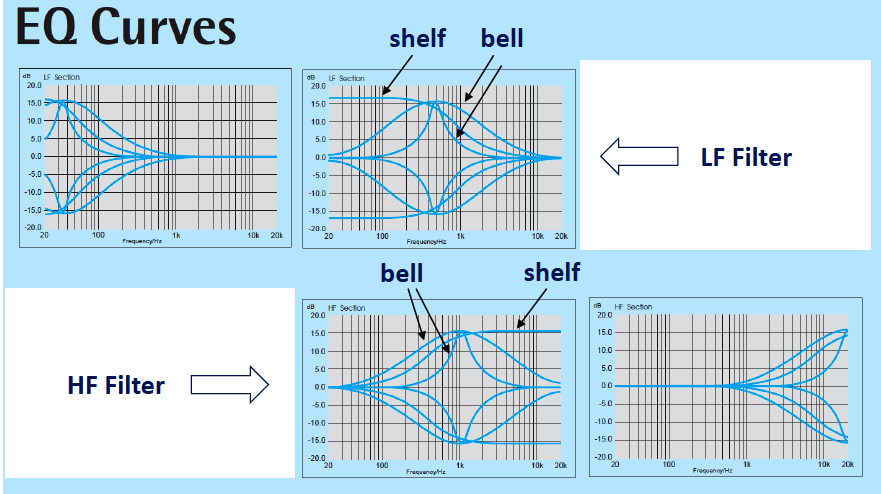
\includegraphics[width=0.90\textwidth]{Mixing_Console_Bell_vs_Shelf.png}
    \caption{Bell and shelf EQ responses available on the low-frequency and high-frequency bands of a parametric equalizer in a professional mixing console}
    \label{fig:bellShelf}
\end{figure}

\paragraph{Insert point} Between the EQ output and the fader, the input strip provides an insert point.
This is a break in the signal path implemented as a send/return loop: the signal leaves the console on the send output, passes through an external processor such as a compressor or gate, and re-enters the channel on the return input.
The insert is typically positioned pre-fader so that the level presented to the external processor does not change when the fader is moved.
Because most external processors use unbalanced \SI{6.35}{\milli\metre} jack connectors while the console's internal signal path is balanced, the insert circuit includes an unbalanced-to-balanced converter on the send and a balanced-to-unbalanced converter on the return, preserving impedance matching and noise immunity across the junction.

% SUGGESTED IMAGE: Insert point send/return circuit with balanced/unbalanced conversion.
% Source: L10 - Soundcraft Series V technical data.pdf
% Filename to add to project: Insert_Point_Circuit.png
\begin{figure}[!htb]
    \centering
    \includegraphics[width=0.90\textwidth]{Soundcraft_Insert_Point.png}
    \caption{Insert point send/return circuit with balanced/unbalanced conversion}
    \label{fig:insertpoint}
\end{figure}

\paragraph{Fader and pan pot} The fader is a logarithmic slide potentiometer that controls the channel's contribution to the mix bus.
Its calibration follows a decibel law aligned with human loudness perception: the nominal unity-gain position is typically marked at \SI{0}{\decibel}, with attenuation below and a small boost range above.
The pan pot (panoramic potentiometer) that follows the fader distributes the signal between the left and right stereo buses, and its electronics are discussed in detail in section \ref{sc:63}.

\section{Electronic Summation: The Summing Amplifier}
\label{sc:62}

A mixing console must combine the outputs of \( N \) independent channels into a single bus signal of the form
\[
y(t) = \sum_{k=1}^{N} a_k \, x_k(t)
\]
where \( a_k \in [0,1] \) is the weight assigned to channel \( k \) by its fader.
The straightforward approach of connecting voltage sources in series to add their amplitudes quickly becomes impractical as the channel count increases.

\subsection{Limitations of Series Voltage Summation}
\label{sc:621}

When \( N \) voltage sources are placed in series, the total voltage swing at the output node grows proportionally with \( N \).
For a console with 48 channels, each carrying a signal of a few volts, the summing node would need to support voltage excursions of tens of volts before any further amplification, straining or exceeding the dynamic range of every downstream stage.
A second, more fundamental problem is that each voltage source in a series connection must be electrically floating with respect to the others: its two terminals cannot both be grounded simultaneously.
In practice every channel in a console shares a common ground reference, which makes true series connection impossible without isolating transformers on each channel, an approach that is prohibitively expensive and bulky at scale.

\begin{figure}[!htb]
    \centering
    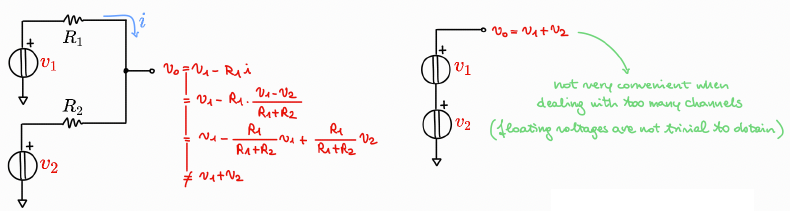
\includegraphics[width=0.90\textwidth]{Mixing_Console_limitation.png}
    \caption{Illustration of the voltage summation problem: series connection causes voltage accumulation proportional to the number of channels and requires floating sources incompatible with a shared ground}
    \label{fig:summationLimit}
\end{figure}

The algebraic result of series summation with resistive coupling confirms the problem.
Applying KVL to two sources \( v_1 \) and \( v_2 \) connected through resistors \( R_1 \) and \( R_2 \) yields
\[
v_0 = v_1 \frac{R_2}{R_1 + R_2} + v_2 \frac{R_1}{R_1 + R_2}
\]
which is a weighted average, not a true sum: \( v_0 \neq v_1 + v_2 \) in general.

\subsection{The Summing Feedback Amplifier}
\label{sc:622}

The correct solution is to convert each channel voltage into a current and sum the currents at a common node.
Since current addition is governed by KCL and does not accumulate voltage, the node voltage remains bounded regardless of how many channels contribute.
The OPAMP in inverting configuration provides both the current-to-voltage conversion via its feedback resistor and a virtual ground at the summing node, as shown in figures \ref{fig:sum1input} and \ref{fig:sum2inputs}.

\begin{figure}[!htb]
    \centering
    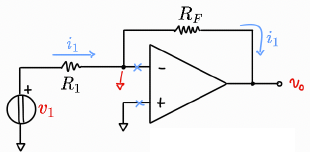
\includegraphics[width=0.40\textwidth]{Mixing_Console_1_input.png}
    \caption{Inverting OPAMP summing stage with a single input: the channel voltage \( v_1 \) is converted into a current \( i_1 = v_1/R_1 \) which flows through the feedback resistor \( R_F \)}
    \label{fig:sum1input}
\end{figure}

\begin{figure}[!htb]
    \centering
    \subfloat[Two-input summing amplifier]{
        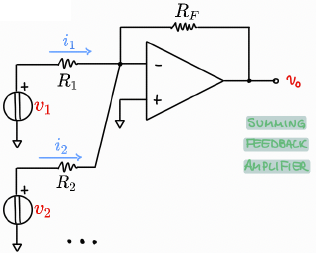
\includegraphics[height=0.20\textheight]{Mixing_Console_2_inputs.png}
    }\hfill
    \subfloat[Current summation concept at the virtual-ground node]{
        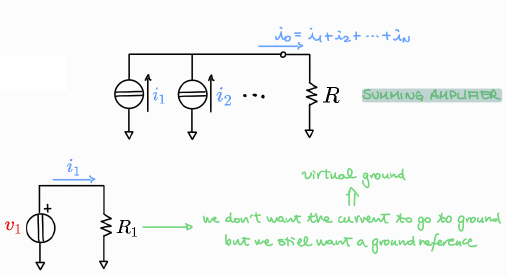
\includegraphics[height=0.20\textheight]{Mixing_Console_Summing_Currents.png}
    }
    \caption{Extension to multiple inputs: by superposition each channel contributes an independent current to the inverting node, and the OPAMP forces their sum through \( R_F \)}
    \label{fig:sum2inputs}
\end{figure}

Applying superposition, the output for two channels follows directly from the ideal OPAMP assumption \( \varepsilon \approx 0 \):
\[
v_0\big|_{v_2=0} = -v_1 \frac{R_F}{R_1}, \qquad v_0\big|_{v_1=0} = -v_2 \frac{R_F}{R_2}
\]
and by linearity
\[
v_0 = -R_F \left( \frac{v_1}{R_1} + \frac{v_2}{R_2} \right)
\]
Extending to \( N \) channels gives the general summing amplifier equation:
\[
V_{out} = -R_F \left( \frac{V_1}{R_1} + \frac{V_2}{R_2} + \cdots + \frac{V_N}{R_N} \right)
\]
The weight \( a_k \) assigned to channel \( k \) is realized by choosing \( R_k = R_F / a_k \), so that the fader's mechanical position sets the effective resistance in the current path.

\paragraph{Loop gain degradation with many channels} A practical limitation arises as \( N \) increases: the feedback factor seen by the OPAMP is
\[
\beta = \frac{R_{IN}}{N \cdot R_F} \propto \frac{1}{N}
\]
so the loop gain \( G_{LOOP} = A_0 \beta \) decreases with the number of channels.
Since correct operation requires \( G_{LOOP} \gg 1 \), very large consoles cascade multiple summing stages rather than connecting all channels to a single amplifier, as illustrated in figure \ref{fig:multiSumLayers}.

\begin{figure}[!htb]
    \centering
    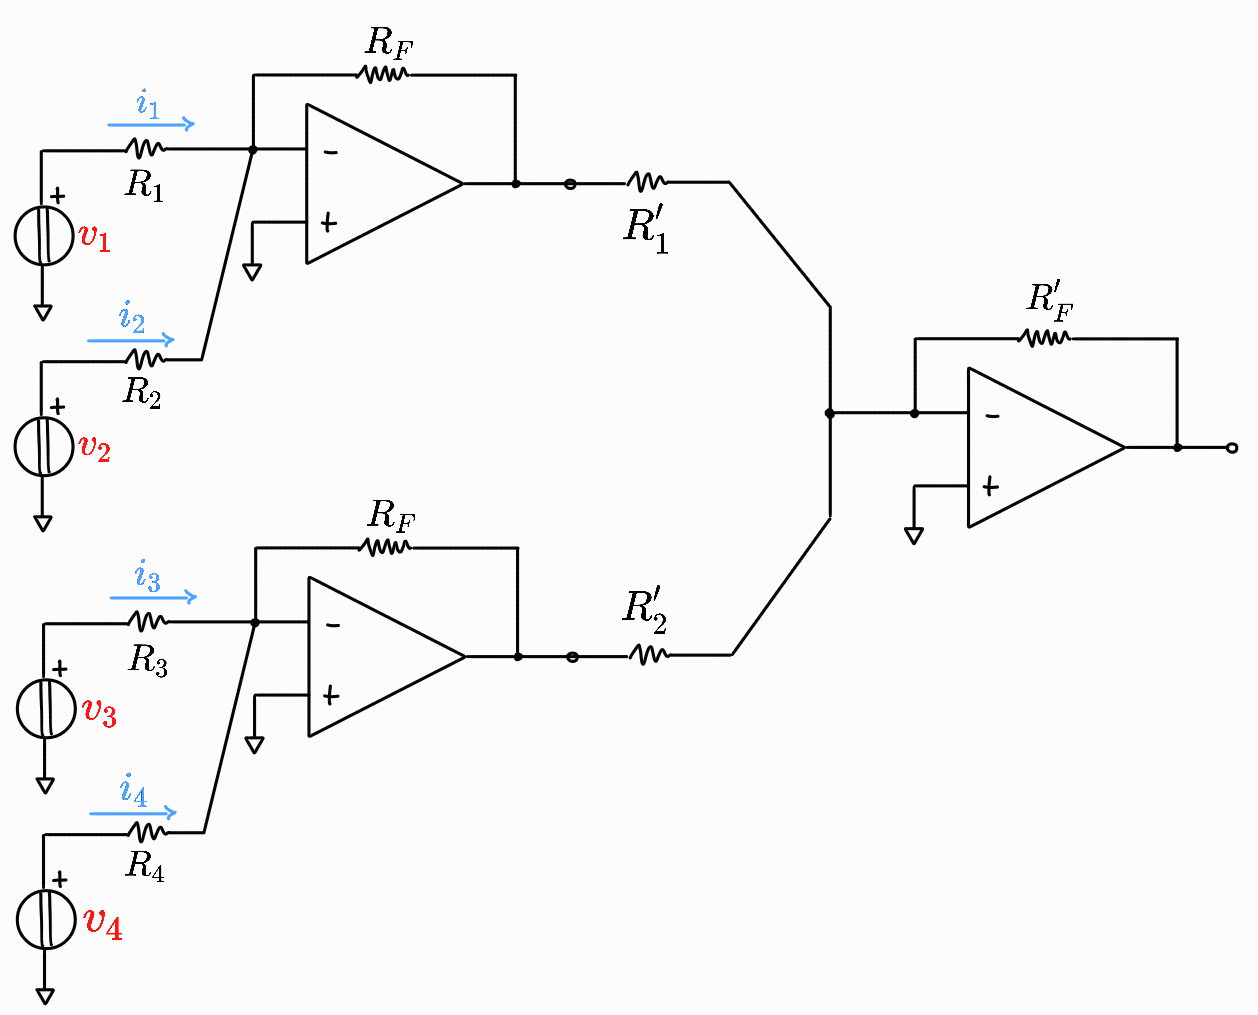
\includegraphics[width=0.65\textwidth]{Mixing_Console_Multiple_Summing_layers.png}
    \caption{Hierarchical summing: channels are first combined in groups of two or four, and the partial sums are then fed to a final summing stage, keeping the loop gain adequate at each level}
    \label{fig:multiSumLayers}
\end{figure}

\subsection{Virtual Ground and Crosstalk Elimination}
\label{sc:623}

The concept of virtual ground is central to understanding why the summing amplifier architecture is superior to any passive network.
Because the OPAMP's negative feedback holds the inverting input at \SI{0}{\volt}, the voltage at the summing node is pinned to ground potential regardless of how many channels are active and what signals they carry.
In real PCB layouts, adjacent signal traces and component leads are inevitably coupled through stray capacitances \( C_{STRAY} \).
Crosstalk arises when a time-varying voltage on one node induces a parasitic current \( i = C_{STRAY} \cdot dV/dt \) into a neighbouring node.
At the virtual-ground node of the summing amplifier the voltage never changes, \( \Delta V_c \approx 0 \), so the numerator of the parasitic current expression vanishes and capacitive crosstalk between channels is effectively eliminated.
This is illustrated in figure \ref{fig:crosstalk}: the stray capacitances that connect the L, R, and C bus nodes to adjacent wiring cannot inject spurious currents because the node they terminate on is held at a constant zero potential.

\begin{figure}[!htb]
    \centering
    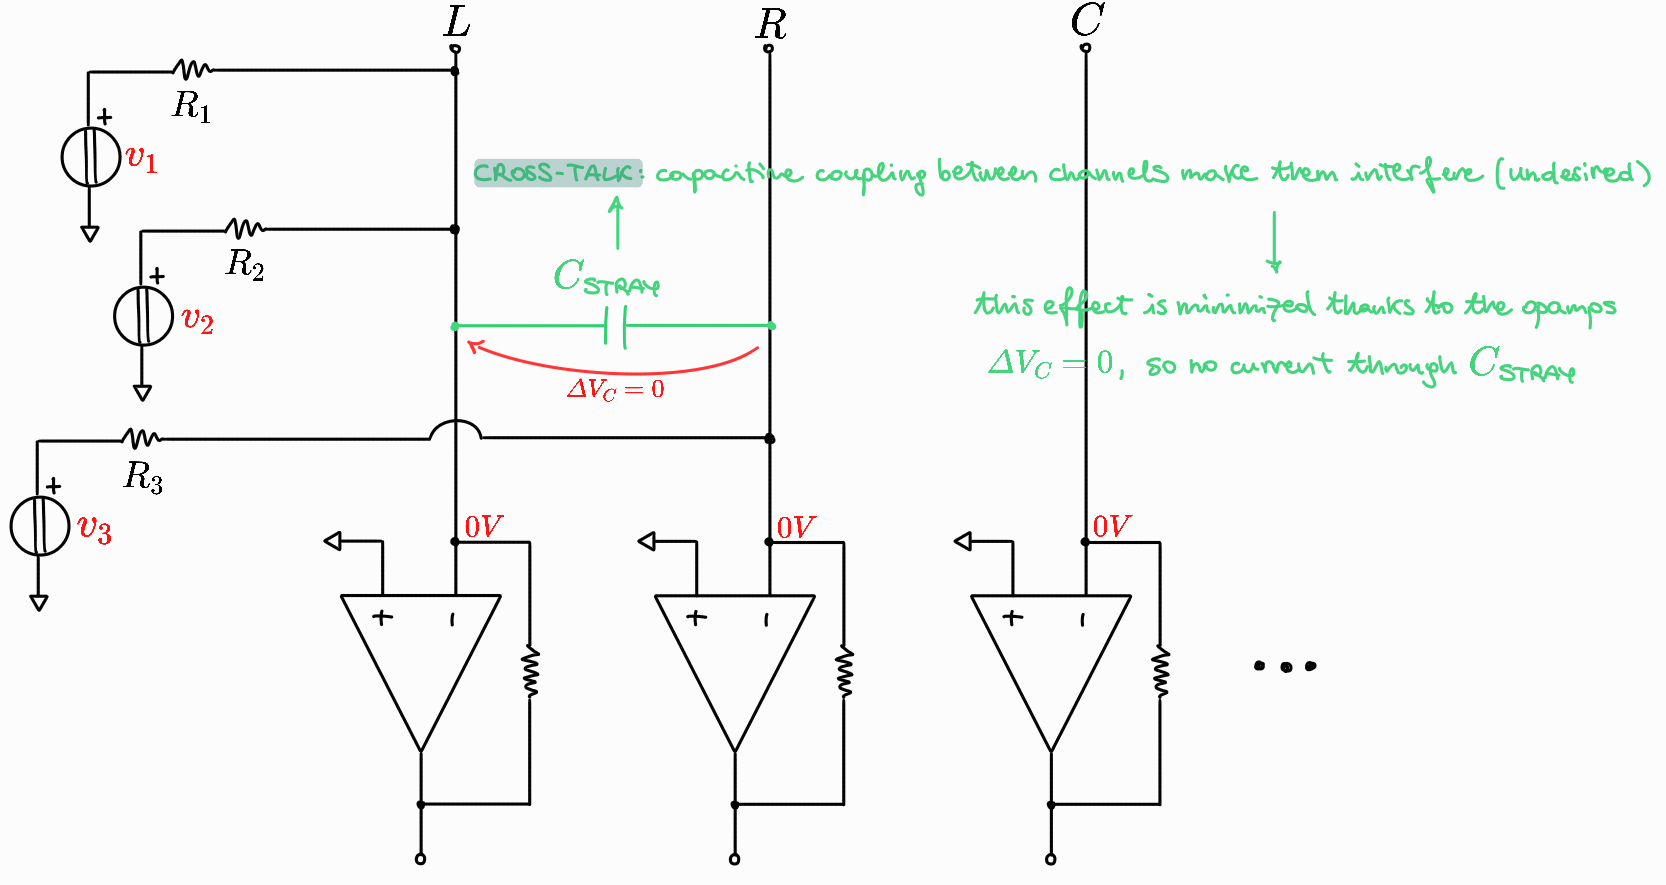
\includegraphics[width=0.90\textwidth]{Mixing_Console_Crosstalk.png}
    \caption{Crosstalk suppression by virtual ground: stray capacitances \( C_{STRAY} \) between the L, R, and C bus conductors inject no parasitic current into the summing node because its voltage is held at \SI{0}{\volt} by the OPAMP feedback}
    \label{fig:crosstalk}
\end{figure}

\section{Panning Potentiometer Electronics}
\label{sc:63}

The panning potentiometer, universally abbreviated as pan pot, controls the lateral position of a mono channel in the stereo image by distributing its signal between the left (L) and right (R) mix buses.
As the knob rotates, the resistance to the left bus increases while the resistance to the right bus decreases by the same amount, so the two sections form a complementary divider.
A unity-gain buffer with output resistance \( R_x \) precedes the potentiometer to isolate the channel from the bus loading.

\begin{figure}[!htb]
    \centering
    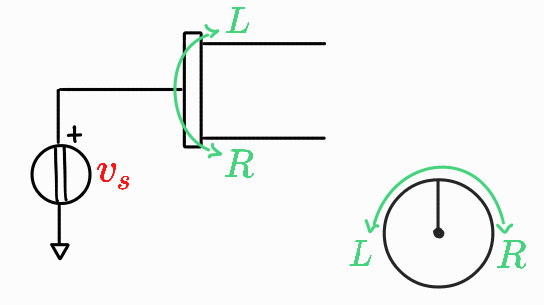
\includegraphics[width=0.30\textwidth]{Pan_Pot_1.png}
    \caption{Model of the panning potentiometer: a voltage buffer feeds the complementary resistive divider that distributes the signal between the L and R buses}
    \label{fig:panPotModel}
\end{figure}

\subsection{Power Analysis and the Center-Position Drop}
\label{sc:631}

The total acoustic power delivered to the stereo bus pair is proportional to the sum of the squared output voltages:
\[
P_{TOT} = P_L + P_R = \frac{V_L^2}{R_x} + \frac{V_R^2}{R_x}
\]
Three canonical positions illustrate the behavior.

\begin{figure}[!htb]
    \centering
    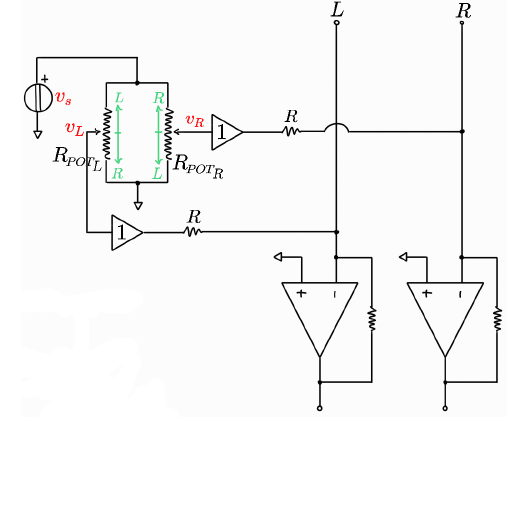
\includegraphics[width=0.55\textwidth]{Pan_Pot_Circuit_1.png}
    \caption{Panning potentiometer circuit: the complementary wiper positions set \( V_L \) and \( V_R \) as a function of the knob angle}
    \label{fig:panPotCircuit}
\end{figure}

\paragraph{Full left} With the knob at the leftmost extreme, all of the source voltage is directed to the left bus and none to the right:
\[
V_L = V_s, \quad V_R = 0 \quad \Rightarrow \quad P_{TOT} = \frac{V_s^2}{R_x}
\]

\paragraph{Full right} Symmetrically, at the rightmost extreme:
\[
V_L = 0, \quad V_R = V_s \quad \Rightarrow \quad P_{TOT} = \frac{V_s^2}{R_x}
\]

\paragraph{Center position} At the geometric center of travel, the potentiometer splits the source voltage equally between the two busses:
\[
V_L = V_R = \frac{V_s}{2} \quad \Rightarrow \quad P_{TOT} = \frac{V_s^2}{4R_x} + \frac{V_s^2}{4R_x} = \frac{V_s^2}{2R_x}
\]
The total power at center is exactly half the power measured at either extreme.
This \( -\SI{3}{\decibel} \) reduction is perceptually significant: a musician panned to center appears to recede in the mix, as if moving further away from the listener, compared to when the same musician is panned hard left or right.
This artifact is known as the center-position power drop.

\begin{figure}[!htb]
    \centering
    \subfloat[Linear potentiometer: power drops at center]{
        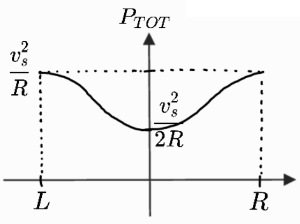
\includegraphics[width=0.40\textwidth]{Pan_Pot_Bad.png}
    }\hfill
    \subfloat[Corrected law: constant power across the pan range]{
        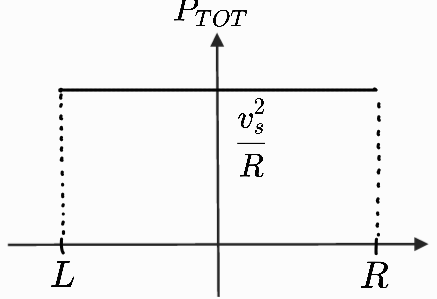
\includegraphics[width=0.40\textwidth]{Pan_Pot_Good.png}
    }
    \caption{Pan pot power curves: the linear potentiometer (left) produces a \( -\SI{3}{\decibel} \) hole at center, while the corrected design (right) maintains constant total power}
    \label{fig:panPotPower}
\end{figure}

\subsection{Constant-Power Panning}
\label{sc:632}

The ideal solution imposes \( P_{TOT} = V_s^2 / R_x \) at every knob position, which requires
\[
V_L^2 + V_R^2 = V_s^2 \quad \forall \, \theta
\]
This constraint is satisfied by the trigonometric law
\[
\begin{cases}
V_L = V_s \sin(\theta) \\
V_R = V_s \cos(\theta)
\end{cases}
\]
since \( \sin^2(\theta) + \cos^2(\theta) = 1 \) by the Pythagorean identity, giving \( P_{TOT} = V_s^2/R_x \) regardless of the pan angle \( \theta \).
This sine-cosine relationship is straightforward to implement in digital mixing consoles, where the pan position is a numerical parameter and the two bus contributions are computed arithmetically.
In analog designs the same effect can be approximated with compensated potentiometers that add bypass resistors \( R_b \) in parallel with each wiper section, shaping the resistance law to follow a curve closer to the trigonometric ideal, as shown in figure \ref{fig:panPotBypass}.

\begin{figure}[!htb]
    \centering
    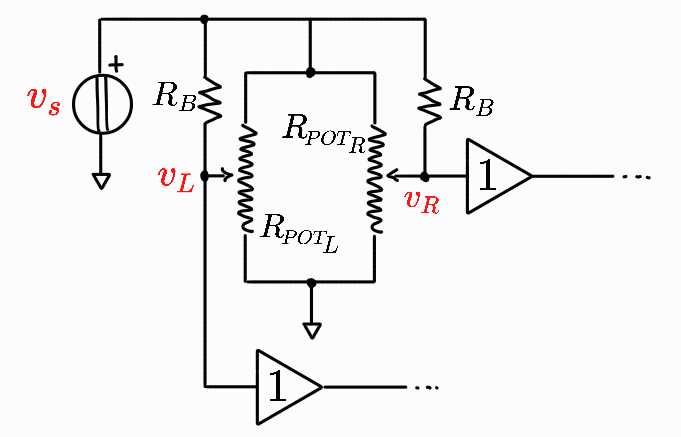
\includegraphics[width=0.40\textwidth]{Pan_Pot_Bypass_Resistor.png}
    \caption{Compensated panning potentiometer: bypass resistors \( R_b \) modify the resistance law to approximate constant-power distribution across the stereo field}
    \label{fig:panPotBypass}
\end{figure}

\section{Routing, Auxiliaries and VCAs}
\label{sc:64}

Once the signal has passed through the fader and pan pot, the channel module provides several routing options that determine where the processed signal is sent.
The three principal destinations in a professional console are the main stereo mix bus, the auxiliary buses, and the group buses; each serves a fundamentally different purpose in the workflow of a session.

\subsection{Console Architecture and Signal Routing}
\label{sc:641}

The overall routing architecture of a professional console is best understood as a matrix: any input channel can be assigned to any combination of output buses through a set of routing switches, as shown in figures \ref{fig:consoleMatrix} and \ref{fig:routingMatrix}.

\begin{figure}[!htb]
    \centering
    \subfloat[Simplified signal flow of a mixing console]{
        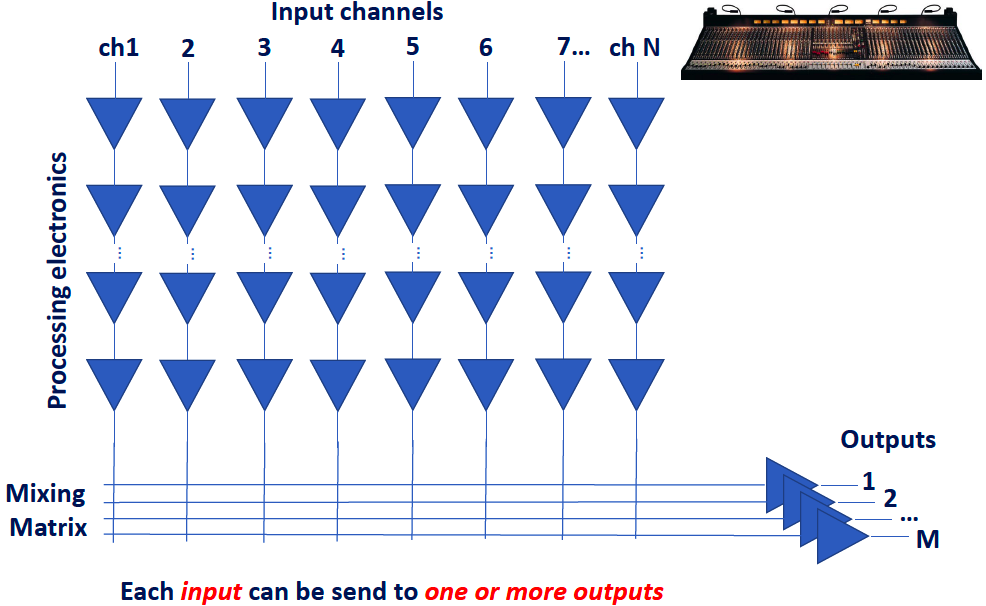
\includegraphics[width=0.45\textwidth]{Mixing_Console_Matrix.png}
    }\hfill
    \subfloat[Routing matrix: each channel feeds selectable output buses]{
        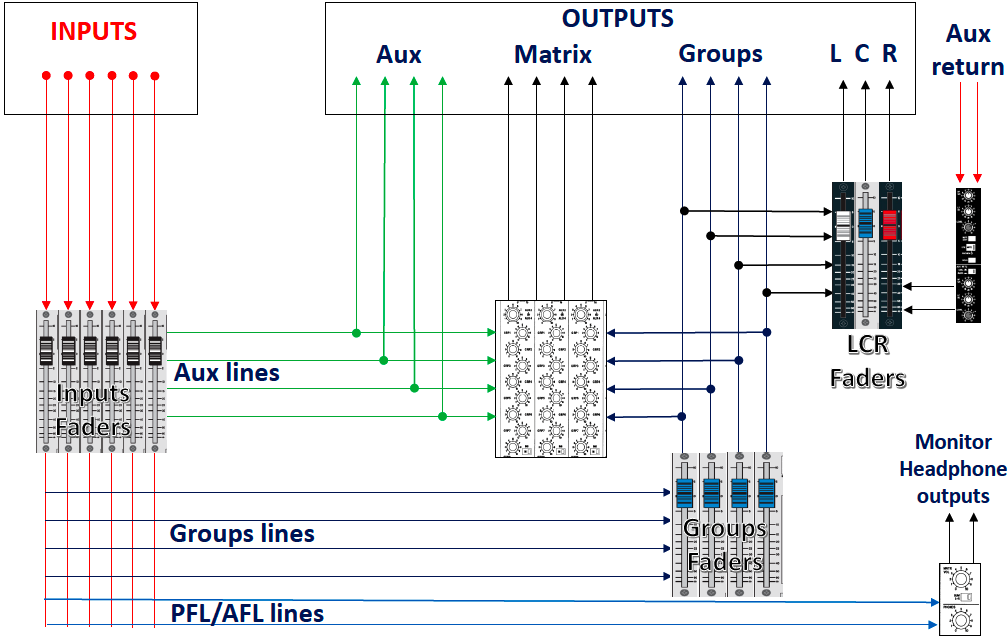
\includegraphics[width=0.45\textwidth]{Mixing_Console_Routing_Matrix.png}
    }
    \caption{Console routing architecture: every input channel can contribute to any output bus through a programmable assignment matrix}
    \label{fig:consoleMatrix}
\end{figure}

\begin{figure}[!htb]
    \centering
    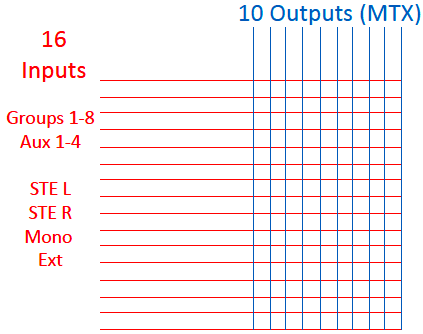
\includegraphics[width=0.40\textwidth]{Mixing_Console_Output_Matrix.png}
    \caption{Simplified schematic of a \( 16 \times 10 \) output matrix section: group and auxiliary outputs are distributed to external destinations}
    \label{fig:routingMatrix}
\end{figure}

\subsection{Auxiliary Lines}
\label{sc:642}

An auxiliary (AUX) bus is a parallel copy of the channel signal that is tapped at a configurable point in the signal path and sent to a dedicated output, independently of the main mix.
Two operating modes are available on most professional consoles.
In pre-fader mode, the AUX tap is taken before the channel fader, so the AUX level is independent of the fader position.
This is the standard configuration for stage monitor mixes: each musician receives a headphone or wedge monitor feed whose level is set by the AUX knob on each channel, and this feed is unaffected when the engineer moves the main fader to adjust the front-of-house balance.
In post-fader mode, the AUX tap is taken after the fader, so the AUX level follows the fader.
This configuration is used for effects sends: when a channel is faded down, its contribution to the reverb or delay bus decreases proportionally, keeping the ratio of dry to wet signal constant.

% SUGGESTED IMAGE: Diagram showing pre-fader and post-fader AUX tap positions.
% Source: L10 - Mixing console.pdf
% Filename to add to project: AUX_Routing_Diagram.png
\begin{figure}[!htb]
    \centering
    \includegraphics[width=0.90\textwidth]{AUX_Mixing_Lines_Diagram.png}
    \caption{Diagram showing pre-fader and post-fader AUX tap positions}
    \label{fig:auxlines}
\end{figure}

\subsection{Groups and Submixes}
\label{sc:643}

A group bus collects the outputs of a set of logically related channels into a sub-mix that is then controlled by a single group fader before being sent to the master bus.
For example, in a live concert setting all drum microphones (kick, snare, hi-hat, toms, overheads) might be assigned to a group bus labeled "Drums": the individual channel faders within that group set the internal balance of the kit, while the group fader sets the overall drum level in the mix without requiring the engineer to move six or eight faders simultaneously.
Groups can be assigned to odd/even bus pairs for stereo submixing, and the group pan switch determines whether the signal is distributed across the stereo field in post-pan-pot mode or sent to the center in pre-pan-pot mode.

\subsection{Voltage Controlled Amplifiers}
\label{sc:644}

In large-format consoles the fader is not the only means of controlling gain.
A Voltage Controlled Amplifier (VCA) is a circuit block whose gain is set by a DC control voltage \( V_c \) rather than by the physical position of a mechanical wiper:
\[
V_{out} = G(V_c) \cdot V_{in}
\]
The audio signal passes through the VCA's electronic gain element without flowing through any potentiometer track or wiper contact, which eliminates the noise and wear associated with high-current mechanical contacts handling audio signals.

% SUGGESTED IMAGE: VCA block diagram showing signal input, control voltage input and signal output.
% Source: L10 - Mixing console.pdf
% Filename to add to project: VCA_Block_Diagram.png
\begin{figure}[!htb]
    \centering
    \subfloat{\includegraphics[width=0.47\textwidth]{VCA_Block_Diagram.png}}\hfill
    \subfloat{\includegraphics[width=0.47\textwidth]{VCA_System_Control_Bus.png}}
    \caption{VCA block diagram showing signal input, control voltage input and signal output}
    \label{fig:VCADiagram}
\end{figure}

\paragraph{VCA groups} The most important operational advantage of VCAs is the ability to assign multiple channels to a VCA group.
When channels 1 through 8 (the rhythm section, for instance) are assigned to VCA group 1, a single master fader generates the control voltage \( V_c \) that simultaneously scales the gain of all eight channels.
Crucially, each channel continues to feed its own individual bus assignments unchanged: the audio routing matrix and the summing amplifiers are not altered in any way.
Only the gain of the audio path through each VCA is modified by \( V_c \), which means the group fader acts as a pure level control with no side effects on panning, auxiliary sends, or any other parameter.
This separation between gain control (via the DC control signal) and signal routing (via the summing bus architecture) is the key architectural advantage of VCA-based console designs over purely mechanical fader grouping, and it is the mechanism that enables the sophisticated automation and recall systems found in modern large-format analog consoles such as the SSL 9000, the Neve VR, and the Soundcraft Series FIVE.

\begin{figure}[!htb]
    \centering
    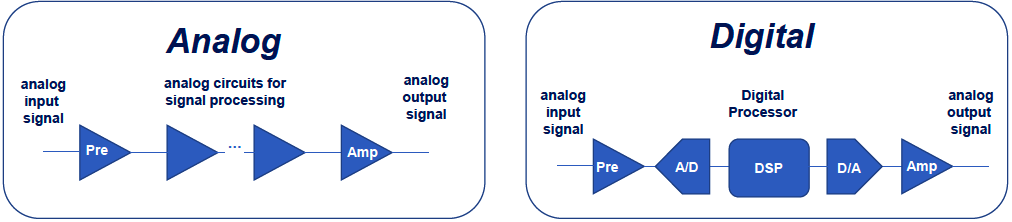
\includegraphics[width=0.90\textwidth]{Analog_vs_Digital_Mixing_Console.png}
    \caption{Comparison between analog and digital console architectures: analog consoles perform all signal processing in the continuous voltage domain, while digital consoles convert signals to the discrete domain and use DSP for all processing}
    \label{fig:analogVsDigital}
\end{figure}

Despite their architectural differences, both analog and digital consoles implement the same conceptual signal flow:
\[
\text{input} \;\rightarrow\; \text{processing} \;\rightarrow\; \text{grouping} \;\rightarrow\; \text{summing} \;\rightarrow\; \text{output}
\]
In the analog domain this chain is realized entirely with operational amplifiers, resistor networks, and VCAs; in the digital domain the same operations are performed by multiply-accumulate instructions in a DSP, but the signal-flow logic and the monitoring requirements are identical.